\documentclass[border=6pt]{standalone}
\usepackage[T1]{fontenc}
\usepackage{tikz}
\usetikzlibrary{automata,positioning,arrows.meta,fit,backgrounds}
\usepackage{helvet}
\renewcommand{\familydefault}{\sfdefault}

\tikzset{
  every state/.style={
    draw, rounded corners=3pt,
    minimum width=2.4cm, minimum height=0.72cm,
    font=\scriptsize\sffamily\bfseries,
    fill=gray!8, thick
  },
  lbl/.style={font=\scriptsize\sffamily, inner sep=2pt},
  arr/.style={-{Stealth[length=5pt]}, thick},
  self/.style={loop, looseness=5}
}

\begin{document}
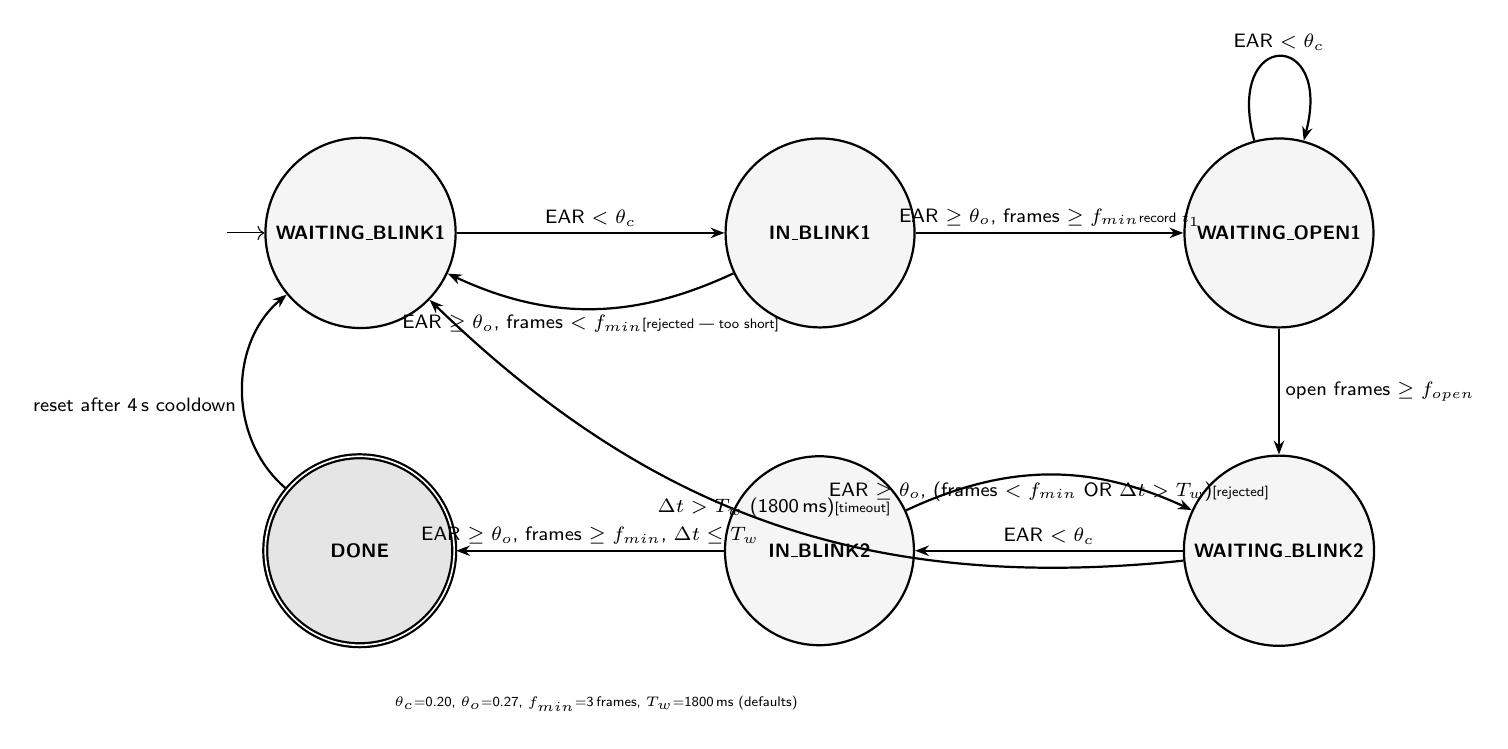
\begin{tikzpicture}[node distance=1.6cm and 3.4cm]

  % States — two rows
  \node[state, initial, initial text={}] (WB1) {WAITING\_BLINK1};
  \node[state, right=of WB1]            (IB1) {IN\_BLINK1};
  \node[state, right=of IB1]            (WO1) {WAITING\_OPEN1};
  \node[state, below=of WO1]            (WB2) {WAITING\_BLINK2};
  \node[state, left=of WB2]             (IB2) {IN\_BLINK2};
  \node[state, accepting,
        left=of IB2,
        fill=gray!20]                   (DONE){DONE};

  % ── Row 1 ──────────────────────────────────────────────────────────────
  \draw[arr] (WB1) -- node[lbl, above]
    {EAR $< \theta_c$} (IB1);

  \draw[arr] (IB1) edge[bend left=25] node[lbl, below]
    {EAR $\geq \theta_o$, frames $< f_{min}$\\[-2pt]\tiny[rejected — too short]}
    (WB1);

  \draw[arr] (IB1) -- node[lbl, above]
    {EAR $\geq \theta_o$, frames $\geq f_{min}$\\[-2pt]\tiny record $t_1$}
    (WO1);

  % self-loop on WAITING_OPEN1
  \draw[arr] (WO1) edge[loop above, looseness=6] node[lbl, above]
    {EAR $< \theta_c$} (WO1);

  % ── Corner ─────────────────────────────────────────────────────────────
  \draw[arr] (WO1) -- node[lbl, right]
    {open frames $\geq f_{open}$} (WB2);

  % ── Row 2 ──────────────────────────────────────────────────────────────
  \draw[arr] (WB2) edge[bend left=25] node[lbl, above]
    {$\Delta t > T_w$ (1800\,ms)\\[-2pt]\tiny[timeout]}
    (WB1);

  \draw[arr] (WB2) -- node[lbl, above]
    {EAR $< \theta_c$} (IB2);

  \draw[arr] (IB2) edge[bend left=25] node[lbl, below]
    {EAR $\geq \theta_o$, (frames $< f_{min}$ OR $\Delta t > T_w$)\\[-2pt]\tiny[rejected]}
    (WB2);

  \draw[arr] (IB2) -- node[lbl, above]
    {EAR $\geq \theta_o$, frames $\geq f_{min}$, $\Delta t \leq T_w$}
    (DONE);

  \draw[arr] (DONE) edge[bend left=50] node[lbl, below left]
    {reset after 4\,s cooldown} (WB1);

  % Caption note
  \node[font=\tiny\sffamily, below=0.5cm of DONE, xshift=3cm]
    {$\theta_c$=0.20, $\theta_o$=0.27, $f_{min}$=3\,frames, $T_w$=1800\,ms (defaults)};

\end{tikzpicture}
\end{document}
